\documentclass[a4paper,openright]{report}
\usepackage[a4paper,top=3cm,bottom=3cm,left=3cm,right=3cm]{geometry} 
\usepackage[fontsize=13pt]{scrextend}
\usepackage[english,russian]{babel}
\usepackage[fixlanguage]{babelbib}
\usepackage[utf8]{inputenc} 
\usepackage[T1]{fontenc}
\usepackage{lipsum}
\usepackage{rotating}
\usepackage{fancyhdr}               
\usepackage{amssymb}
\usepackage{amsmath}
\usepackage{amsthm}         
\usepackage{graphicx}
\usepackage[dvipsnames]{xcolor}         
\usepackage{listings}      
\usepackage[svgnames]{xcolor}
\usepackage{hyperref} 
\usepackage[normalem]{ulem}
\setlength{\parindent}{0ex}
\usepackage{diagbox}
\usepackage{graphicx}
\usepackage{color,colortbl}
\definecolor{royalblue}{RGB}{65,105,225}
\definecolor{blue}{RGB}{197,221,246}
\definecolor{green}{RGB}{33,183,98}
% -----------------------------------------------------------------

\pagestyle{fancy}
\fancyhf{}
\lhead{\rightmark}
\rhead{\textbf{\thepage}}
\fancyfoot{}
\setlength{\headheight}{12.5pt}


\fancypagestyle{plain}{
  \fancyfoot{}
  \fancyhead{}
  \renewcommand{\headrulewidth}{0pt}
}


\lstdefinestyle{codeStyle}{
    commentstyle=\color{green},
    keywordstyle=\color{royalblue},
    numberstyle=\tiny\color{gray},
    stringstyle=\color{green},
    basicstyle=\ttfamily\footnotesize,
    breakatwhitespace=false,     
    breaklines=true,                 
    captionpos=b,                    
    keepspaces=true,                 
    numbers=left,                    
    numbersep=5pt,                  
    showspaces=false,                
    showstringspaces=false,
    showtabs=false,
    tabsize=2
} \lstset{style=codeStyle}

\lstdefinestyle{longBlock}{
    commentstyle=\color{teal},
    keywordstyle=\color{Magenta},
    numberstyle=\tiny\color{gray},
    stringstyle=\color{violet},
    basicstyle=\ttfamily\scriptsize,
    breakatwhitespace=false,         
    breaklines=true,                 
    captionpos=b,                    
    keepspaces=true,                 
    numbers=left,                    
    numbersep=5pt,                  
    showspaces=false,                
    showstringspaces=false,
    showtabs=false,                  
    tabsize=2
} \lstset{style=codeStyle}

\lstset{aboveskip=20pt,belowskip=20pt}


\hypersetup{
    colorlinks,
    linkcolor=CornflowerBlue,
    citecolor=CornflowerBlue
}


\newtheorem{definition}{Definizione}[section]
\newtheorem{theorem}{Teorema}[section]
\providecommand*\definitionautorefname{Definizione}
\providecommand*\theoremautorefname{Teorema}
\providecommand*{\listingautorefname}{Listing}
\providecommand*\lstnumberautorefname{Linea}

\raggedbottom
% -----------------------------------------------------------------
\begin{document}

\begin{titlepage}
\begin{figure}[!htb]
    \centering
    
\includegraphics[keepaspectratio=true,scale=1.2]{images/title/msu_logo.png}
\end{figure}

\begin{center}
    МИНИСТЕРСТВО ОБРАЗОВАНИЯ И НАУКИ \\РОССИЙСКОЙ ФЕДЕРАЦИИ
    \vspace{5mm}
    \\ \large{МОСКОВСКИЙ ГОСУДАРСТВЕННЫЙ УНИВЕРСИТЕТ\\ им М.В.Ломоносова}
    \vspace{5mm}
    \\Механико-математический факультет \\ Кафедра теории вероятностей
\end{center}

\vspace{15mm}
\begin{center}
    {\LARGE{\textbf{Курсовая работа} \\ \vspace{3mm} Нетранзитивные наборы финансовых стратегий на фондовом рынке }}
\end{center}
\vspace{30mm}

\begin{minipage}[t]{0.47\textwidth}
	{\large{\textbf{Выполнил:}}{\normalsize\vspace{3mm}
	\\ \large{Cтудент 5 курса 531 группы \\ Ковальчук А.А.} \normalsize\vspace{3mm}}}
\end{minipage}
\hfill
\begin{minipage}[t]{0.47\textwidth}\raggedleft
	{\large{\textbf{Научный руководитель:}}{\normalsize\vspace{3mm} 
	\\ \large{Доцент кафедры теории веротностей Лебедев А.В.}}}
\end{minipage}

\vspace{20mm}
\hrulefill
\\\centering{Москва, 2022 г.}

\end{titlepage}
\tableofcontents
\chapter{Введенеие}

Фондовый рынок - это неотёемлемая часть экономического сектора уже многие столетия. Область активно развивается и вовлекает все больше и больше людей с каждым годом. Безусловно, для анализа и прогнозирования поведения активов используют методы математического моделирования. В этой работе будет разобрано одно из свойств стратегий, которые могут быть применены для торговли активами на фондовом рынке. Перейдем к проблематике.

\section{Проблематика}

В статье Токарева Сергея Степановича “Нетранзитивный лохотрон на фондовом рынке” утверждается существование нетранзитивных наборов финансовых стратегий$^{[1]}$. Одна стратегия считается лучше другой, если она чаще дает больший результат. Автор утверждает, что существует пример стратегий, при котором первая стратегия лучше второй (в смысле описанном выше), вторая стратегия лучше третьей, но неверно, что первая стратегия лучше стратегии три, то есть:

\begin{center}
($s_1 \succ s_2) \bigwedge (s_2 \succ s_3) \nRightarrow s_1 \succ s_3$
\end{center}

\section{Описание стратегий}

Будем рассматривать 3 стратегии:
\begin{enumerate}
\item стратегия $s_1$(первая): продажа акций производится в самом начале торгового дня по текущей биржевой цене (чистая прибыль всегда равна нулю).
\item стратегия $s_2$ (вторая): продажа акций производится в тот момент, когда их цена впервые снизится более чем на $a\%$, либо поднимется более чем на $b\%$ от их стоимости на начало торгового дня. Если же цена за весь день ни разу не достигнет ни одного из указанных уровней, то продажа производится в конце торгов по текущей цене.
\item стратегия $s_3$ (третья): продажа акций производится в тот момент, когда их цена впервые снизится более чем на $c\%$, либо поднимется более чем на $d\%$ от их стоимости на начало торгового дня. Если опять же цена ни разу за весь день не достигнет ни одного из указанных критических уровней, то продажа производится в конце торгов по текущей цене.
\end{enumerate}

\section{Постановка задачи}
Необходимо дать более точное математическое обоснование данного вопроса, изучить зависимость вероятностей от пороговых значений, разобраться, когда нетранзитивность в этой системе должна проявляться в большей степени, а когда в меньшей. Помимо этого важной задачей будет произвести численный эксперимент на реальных данных и проверить, выполняться ли теоритические выводы на практике.


\chapter{Теоретическое обоснование}

Эта глава будет посвещена теоретическому исследованию вопроса нетранзитивности. Будет произведен расчет необходимых вероятностей и исследование силы нетранзитивности полученных соотношений.

\section{Причина отсутствия транзитивности}

Приведем обоснование при $a = 0.6\%$, $b = 0.3\%$, $c = 0.3\%$, $d = 0.6\%$. Здесь $a, b, c, d$ аналогичны тем, что были введены в предыдущей главе.
\smallskip
\smallskip

Вероятность того, что при работе с одними и теми же акциями на одном и том же временном интервале вторая стратегия приведет к реализации бумаг по более высокой цене, чем первая, равна приблизительно $2 \over 3$ или $66.7\%$. Это следует из того, что ожидаемая вероятность изменения на $0.6\%$ должна быть в два раза меньше, чем на $0.3\%$. Таким образом, вторая стратегия в указанном смысле оказывается лучше первой, то есть доминирует над ней. 
\smallskip
\smallskip

С другой стороны, вероятность того, что при аналогичных условиях третья стратегия позволит продать бумаги дороже, в сравнении со второй, также превышает $50\%$. Это следует из того, что на росте акции мы с большей вероятностью зафиксируем большую прибыль, а на падении меньший убыток. То есть третья стратегия, в свою очередь, доминирует над второй.
\smallskip
\smallskip

Предполагая транзитивность определенного нами отношения доминирования, можно подумать, что третья стратегия является самой предпочтительной из всех трех. Однако эта гипотеза не будет соответствовать действительности, так как на самом деле первая стратегия обеспечивает более высокую цену продажи по сравнению с третьей опять же с вероятностью примерно $66.7\%$. Далее мы подтвердим это строго.

\section{Расчет вероятностей}

Введем случайные величины, соответствующие прибыли для каждой из трёх стратегий. Введем их для удобства вычислений следующим образом:

\begin{center}
$X_1 \equiv 0$, 
$X_2$ = 
 \begin{cases}
   -a, &\text{с вер. $p_{-}(a, b)$}\\
   $\hspace{10pt}$ b, &\text{с вер. $p_{+}(a, b)$}
 \end{cases},
$X_3$ = 
 \begin{cases}
   -c, &\text{с вер. $p_{-}(c, d)$}\\
   $\hspace{9pt}$d, &\text{с вер. $p_{+}(c, d)$}
 \end{cases}
\smallskip
\end{center}


Тогда будет верно, что $P(X_1 < X_2) = p_{+}(a,b)$, $P(X_2 < X_1) = p_{-}(a,b)$. Аналогично $P(X_1 < X_3) = p_{+}(c,d)$, $P(X_3 < X_1) = p_{-}(c,d)$. Вычислим $p_{+}(a,b), p_{-}(a,b)$, вероятности $p_{+}(c,d), p_{-}(c,d)$ будут после этого определены автоматически.
\smallskip
\smallskip

Пусть $S_0$ - это стоимость акции в начале торгового дня. Пусть $A = {a\over{100\%}}$, $B = {b\over{100\%}}$, $p_{+}(a,b):= p_{+}$, $p_{-}(a,b):= p_{-}$. 
\smallskip
\smallskip

Будем использовать теорему Дуба об остановке$^{[2]}$. Тогда имеем, что:

\begin{center}
$S_0 = p_{+}S_0(1+B) + p_{-}S_0(1-A)$

$1 = p_{+}(1+B) + (1-p_{+})(1-A)$

$p_{+} = {A\over{A + B}} = {a\over{a + b}}, p_{-} = {b\over{a + b}}$
\end{center}

Тогда в примере, который мы описывали в предыдущей главе, будем иметь, что $p_{+}(0.6, 0.3) = {2\over{3}}, p_{-}(0.6, 0.3) = {1\over{3}}$.
\smallskip
\smallskip

Итого имеем, что:
\begin{center}
$p_{+}(a,b) = {a\over{a + b}}, p_{-}(a,b) = {b\over{a + b}}, p_{+}(c,d) = {c\over{c + d}}, p_{-}(c,d) = {d\over{c + d}}$
\end{center}


Теперь приступим к нахождению $P(X_2 < X_3)$. Сразу отметим, что случайные величины $X_2$ и $X_3$ зависимы, поэтому заполним таблицу вероятностей изменения цены акций ниже (не теряя общности будем считать, что $c < a$, $b < d$):

\begin{center}
   \begin{tabular}{|l|c|c|}\hline
    \diagbox[width=4em]{X_3}{X_2}&
      $-a$ & $b$ \\ \hline
      $-c$ & $p_{--}$ & $p_{+-}$ \\ \hline
      $d$ & $p_{-+}$ & $p_{++}$\\ \hline
    \end{tabular} 
\end{center}

Тогда будет верно, что $P(X_2 < X_3) = p_{--} + p_{-+} + p_{++}$. 
\smallskip
\smallskip

Верно, что $p_{--} = p_{-}(a, b) = {b\over{a + b}}$. Расчитывая вероятность таким образом, мы уверены, что цена акции не выйдет за полосу равную $b$ (а значит и $d$) и автоматически пересечет полосу $-c$.
\smallskip
\smallskip

Далее рассмотрим $p_{-+}$. Эта вероятность равна нулю, так как если $X_2 = -a$, то $X_3 = -c$, так как $c < a$. С другой стороны, если $X_3 = d$, то $X_2 = b$, так как $b < d$.
\smallskip
\smallskip

Наконец рассмотрим $p_{++}$. Аналогично рассуждению для $p_{--}$ будем иметь, что $p_{++} = p_{+}(c, d) = {c\over{c + d}}$. Имеем следующее: 


\begin{center}
    $P(X_2 < X_3) =  {b\over{a + b}} + {c\over{c + d}}$
\end{center}

Тогда получаем, что условие нетранзитивности можно записать в следующем виде:


\begin{center}
    $P(X_1 < X_2) > {1\over 2}, P(X_2 < X_3) > {1\over 2}, P(X_3 < X_1) > {1\over 2}$
    
    ${a\over{a + b}} > {1\over 2}, {b\over{a + b}} + {c\over{c + d}} > {1\over 2}, {d\over{c + d}} > {1\over 2}$
\end{center}

Еще раз проверим условие нетранзитивности для $a = 0.6$, $b = 0.3$, $c = 0.3$, $d = 0.6$.

\begin{center}
    ${a\over{a + b}} = {2\over 3} > {1\over 2}, {b\over{a + b}} + {c\over{c + d}} = {2\over{3}} > {1\over{2}}, {d\over{c + d}} = {2\over 3} > {1\over 2}$
\end{center}

Нетранзитивность доказана. Уделим внимание еще одному моменту. Докажем, что сумма вероятностей в таблице будет равна $1$. Для этого сначала вычислим  $p_{+-}$.
\smallskip
\smallskip

Необходимо рассмотреть два случая. Первый: стоимость сначала опускается до $-c$, а потом поднимается до $b$. Второй: стоимость сначала поднимается на $b$, а потом опускается на $-c$. Первая вероятность может быть вычислена так:  ${b\over{b + c}} * {a-c\over{a + b}}$. Вторая вероятность вычисляется так: ${c\over{b + c}} * {d-b\over{d + c}}$. Итого получаем, что $p_{+-} = {b(a-c)\over{(a + b)(b + c)}} + {c(d-b)\over{(b + c)(d + c)}}$. Перейдем к проверке:

\begin{center}
    $p_{--} + p_{-+} + p_{+-} + p_{++} = {b\over{a + b}} + {b(a-c)\over{(a + b)(b + c)}} + {c(d-b)\over{(b + c)(d + c)}} + {c\over{c + d}} = $
    
    ${b(b+a)\over{(a + b)(b+c)}} + {c(d+c)\over{(b + c)(c+d)}} = {b\over{b + c}} + {c\over{b + c}} = 1$
\end{center}
Равенство суммы вероятностей единицы выполнено. Теперь перейдем к решению оптимизационной задачи.

\section{Решение оптимизационной задачи}

Перейдем к исследованию полученных соотношений. Будем максимизировать силу нетранзитивности, а именно: 

\begin{center}
$min((P(X_1 < X_2), P(X_2 < X_3), P(X_3 < X_1)) \to max$

$min({a\over{a + b}}, {b\over{a + b}} + {c\over{c + d}}, {d\over{c + d}}) \to max$

$x := {a\over{a + b}}, y:= {d\over{c + d}}, 0 < x < 1, 0 < y < 1$

$min(x, 2 - x - y, y) \to max$

\end{center}

Минимум левого вырежния можно рассмотреть, как минимум из трех функций $f_1(x, y) = x, f_2(x,y) = 2 - x - y, f_3(x, y) = y$. Построим графики этих функций в одной системе координат и оставим их части соответствующие $min(f_1, f_2, f_3)$:

\begin{center}
    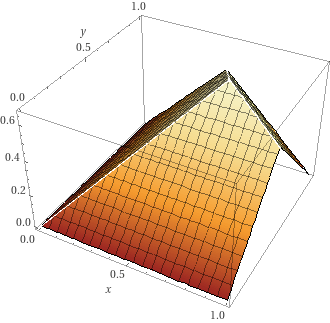
\includegraphics[keepaspectratio=true,scale=1]{images/chapter1/1.png}
\end{center}


Из графика видно, что максимум достигается в точке пересечения трех плоскостей, значит, надо приравнять все три функции, то есть $x = 2 - x - y = y$. Отсюда получаем что $x = y = {2 \over 3}$. Таким образом $({2 \over 3}, {2 \over 3})$  - точка максимума. 
\smallskip
\smallskip

Возвращаясь к изначальным переменным имеем, что сила нетранзитивности максимальна при $a = 2b$, $d = 2c$ сила нетранзитивности будет максимальной. Теперь перейдем к практической части.

\chapter{Численный эксперимент}

В этой главе мы исследуем свойство нетранзитивности на реальных данных. Проведем численный эксперимент при $a = d$, $b = c$ (для простоты анализа).
То есть одна стратегия закрывалась в плюс на таком же проценте, как и другая в минус, и наоборот. Эксперимент будем проводить на акциях Сбербанка за 2017, 2018, 2019, 2020, 2021 (ticker = SBER)$^{[3]}$.
\section{Описание эксперимента}

Будем считать, что одна стратегия лучше другой, если она чаще дает больший результат. Поэтому наша цель, подтвердить, что приведенные ранее соотношения для стратегий будут выполняться. Для агрегирования данных будем использовать язык Python и библиотеку Pandas. Код будет приведен в следующей главе.
\smallskip
\smallskip

Результаты приведем в таблицах: по строкам укажем всевозможные исходы (их 9 штук), по столбцам обозначим годы. В пересечении строк и столбцов укажем процент, соответсвующий кажому исходу по годам.
\smallskip
\smallskip

Для первого эксперимента $a = d = 0.6$, $b = c = 0.3$. Результат:

\begin{table}[!ht]
\centering
\begin{tabular}{|l|l|l|l|l|l|}
\hline
     & 2017 & 2018 & 2019 & 2020 & 2021 \\ \hline
    s1 > s2 & 36.9 & 31.9 & 32.9 & 36.8 & 39.4 \\ \hline
    \rowcolor{blue}s1 > s3 & 65.5 & 63.0 & 63.9 & 66.8 & 74.3 \\ \hline
    \rowcolor{blue}s2 > s1 & 63.1 & 68.1 & 67.1 & 63.2 & 60.6 \\ \hline
    s2 > s3 & 29.0 & 31.1 & 31.3 & 30.0 & 35.0 \\ \hline
    s3 > s1 & 34.5 & 37.0 & 36.1 & 33.2 & 25.7 \\ \hline
    \rowcolor{blue}s3 > s2 & 67.1 & 59.4 & 66.7 & 61.6 & 62.4 \\ \hline
    s1 == s2 & 0.0 & 0.0 & 0.0 & 0.0 & 0.0 \\ \hline
    s1 == s3 & 0.0 & 0.0 & 0.0 & 0.0 & 0.0 \\ \hline
    s2 == s3 & 4.0 & 9.4 & 2.0 & 8.4 & 2.7 \\ \hline
    Количество дней & 252 & 254 & 252 & 250 & 226 \\ \hline
\end{tabular}
\end{table}

\textbf{Вывод:} за все годы наблюдается эффект нетранзитивности. Из таблицы видно, что $s_2 > s_1$ (действительно примерно в $2 \over 3$ случаев) и  $s_1 > s_3$ (также примерно в $2 \over 3$ случаев), но соотношение, что $s_2 > s_3$  является неверным.
\smallskip
\smallskip

 Далее возьмем $a = d = 0.4$, $b = c = 0.2$. Результат:
 \begin{table}[!ht]
    \centering
    \begin{tabular}{|l|l|l|l|l|l|}
    \hline
         & 2017 & 2018 & 2019 & 2020 & 2021 \\ \hline
        s1 > s2 & 40.1 & 35.0 & 38.1 & 38.4 & 42.0 \\ \hline
        \rowcolor{blue}s1 > s3 & 63.9 & 58.3 & 63.9 & 64.8 & 68.6 \\ \hline
        \rowcolor{blue}s2 > s1 & 59.9 & 65.0 & 61.9 & 61.6 & 58.0 \\ \hline
        s2 > s3 & 23.8 & 23.2 & 25.8 & 26.4 & 26.5 \\ \hline
        s3 > s1 & 36.1 & 41.7 & 36.1 & 35.2 & 31.4 \\ \hline
        \rowcolor{blue}s3 > s2 & 59.1 & 53.1 & 65.5 & 54.0 & 70.4 \\ \hline
        s1 == s2 & 0.0 & 0.0 & 0.0 & 0.0 & 0.0 \\ \hline
        s1 == s3 & 0.0 & 0.0 & 0.0 & 0.0 & 0.0 \\ \hline
        s2 == s3 & 17.1 & 23.6 & 8.7 & 19.6 & 3.1 \\ \hline
        Количество дней & 252 & 254 & 252 & 250 & 226 \\ \hline
    \end{tabular}
\end{table}

\textbf{Вывод:} при изменении параметров второй и третьей стратегии эффект нетранзитивности сохраняется.
\smallskip
\smallskip

 Далее возьмем $a = d = 0.5$, $b = c = 0.25$. Результат:
 \begin{table}[!ht]
    \centering
    \begin{tabular}{|l|l|l|l|l|l|}
    \hline
         & 2017 & 2018 & 2019 & 2020 & 2021 \\ \hline
        s1 > s2 & 36.1 & 32.7 & 36.1 & 37.2 & 43.8 \\ \hline
        \rowcolor{blue}s1 > s3 & 65.9 & 59.4 & 62.7 & 66.0 & 71.2 \\ \hline
        \rowcolor{blue}s2 > s1 & 63.9 & 67.3 & 63.9 & 62.8 & 56.2 \\ \hline
        s2 > s3 & 29.8 & 26.8 & 27.0 & 28.8 & 27.4 \\ \hline
        s3 > s1 & 34.1 & 40.6 & 37.3 & 34.0 & 28.8 \\ \hline
        \rowcolor{blue}s3 > s2 & 60.3 & 58.7 & 69.8 & 60.0 & 69.0 \\ \hline
        s1 == s2 & 0.0 & 0.0 & 0.0 & 0.0 & 0.0 \\ \hline
        s1 == s3 & 0.0 & 0.0 & 0.0 & 0.0 & 0.0 \\ \hline
        s2 == s3 & 9.9 & 14.6 & 3.2 & 11.2 & 3.5 \\ \hline
        Количество дней & 252 & 254 & 252 & 250 & 226 \\ \hline
    \end{tabular}
\end{table}

\textbf{Вывод:} при изменении параметров второй и третьей стратегии эффект нетранзитивности сохраняется.

\newpage
Последний эксперимент: $a = d = 2$, $b = c = 1$. Результат:

\begin{table}[!ht]
    \centering
    \begin{tabular}{|l|l|l|l|l|l|}
    \hline
         & 2017 & 2018 & 2019 & 2020 & 2021 \\ \hline
        s1 > s2 & 25.4 & 27.6 & 25.0 & 26.4 & 28.3 \\ \hline
        \rowcolor{blue}s1 > s3 & 69.8 & 74.4 & 71.8 & 70.8 & 70.8 \\ \hline
        \rowcolor{blue}s2 > s1 & 74.2 & 72.4 & 75.0 & 73.6 & 71.7 \\ \hline
        \rowcolor{blue}s2 > s3 & 50.8 & 51.6 & 49.6 & 49.2 & 46.9 \\ \hline
        s3 > s1 & 29.8 & 25.6 & 27.8 & 29.2 & 29.2 \\ \hline
        s3 > s2 & 22.2 & 34.3 & 13.5 & 30.0 & 20.8 \\ \hline
        s1 == s2 & 0.4 & 0.0 & 0.0 & 0.0 & 0.0 \\ \hline
        s1 == s3 & 0.4 & 0.0 & 0.4 & 0.0 & 0.0 \\ \hline
        s2 == s3 & 27.0 & 14.2 & 36.9 & 20.8 & 32.3 \\ \hline
        Количество дней & 252 & 254 & 252 & 250 & 226 \\ \hline
    \end{tabular}
\end{table}

\textbf{Вывод:} при изменении параметров нетранзитивность сохраняется, только в более слабом смысле: не вероятность выигрыша больше половины, а вероятность выигрыша больше вероятности проигрыша (поскольку ничьи отнимают часть полной вероятности). Также можно заметить рост равенства стратегий $s_2$ и $s_3$.

\section{Графическая эллюстрация}
Дополнительно рассмотрим на графиках всевозможные варианты реализации стратегий $s_2$ и $s_3$ для $a = d = 0.6$, $b = c = 0.3$. Всего есть 9 всевозможных реализаций (как уже было указано ранее). Опишем их и приведем графики ниже:

\begin{enumerate}
    \item $s_2$ продажа на повышение, $s_3$ продажа на повышение (рис. 3.1)
    \item $s_2$ продажа на повышение, $s_3$ продажа на понижение (рис. 3.2)
    \item $s_2$ продажа на повышение, $s_3$ продажа в конце дня (рис. 3.3)
    \item $s_2$ продажа на понижение, $s_3$ продажа на повышение (не реализуется)
    \item $s_2$ продажа на понижение, $s_3$ продажа на понижение (рис. 3.4)
    \item $s_2$ продажа на понижение, $s_3$ продажа в конце дня (не реализуется)
    \item $s_2$ продажа в конце дня, $s_3$ продажа на повышение (не реализуется)
    \item $s_2$ продажа в конце дня, $s_3$ продажа на понижение (рис. 3.5)
    \item $s_2$ продажа в конце дня, $s_3$ продажа в конце дня (рис. 3.6)
\end{enumerate}
\smallskip

Сразу отметим, что случаи, описанные под буквами г, е, ж не реализуются. Случай, описанный под пунктом и), также не был найден для выбранных  $a, b, c, d$, но при увеличении этих значений на незначительную величину приведет также к реализации этого случая (см. рис. 6). 

\begin{center}
    \begin{figure}[h]
        \centering
        \caption{$s_2$ продажа на повышение, $s_3$ продажа на повышение}
        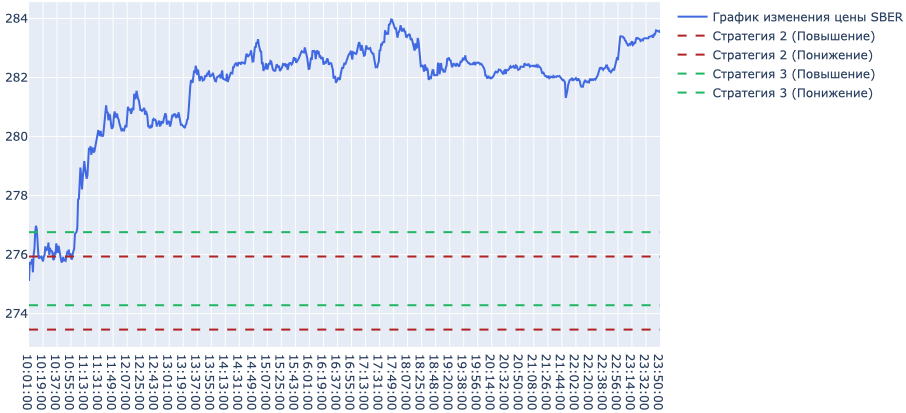
\includegraphics[keepaspectratio=true,scale=0.35]{images/chapter3/upup.png}
        
        \caption{$s_2$ продажа на повышение, $s_3$ продажа на понижение}
        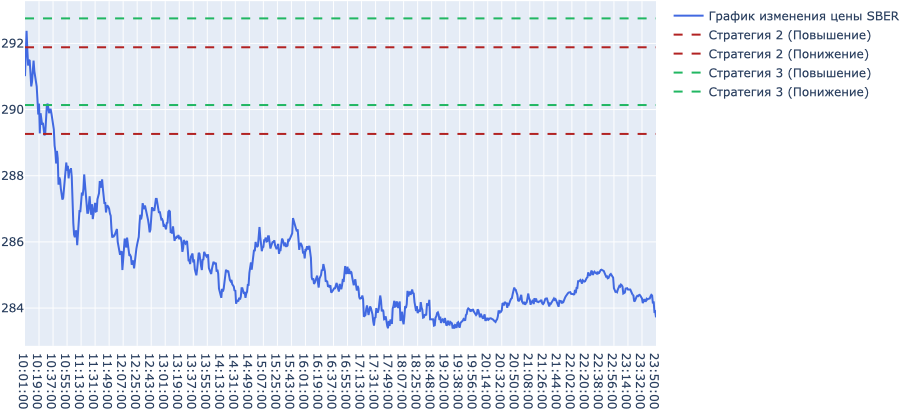
\includegraphics[keepaspectratio=true,scale=0.35]{images/chapter3/updown.png}
        
        \caption{$s_2$ продажа на повышение, $s_3$ продажа в конце дня}
        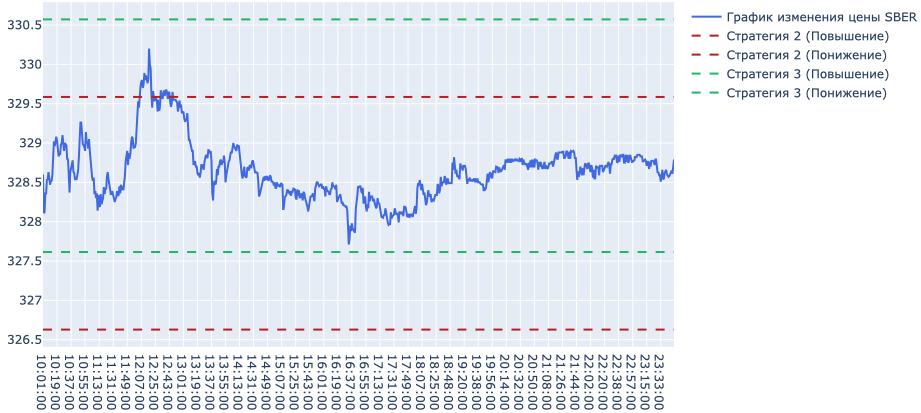
\includegraphics[keepaspectratio=true,scale=0.35]{images/chapter3/upzero.png}
    \end{figure}
\end{center}


Здесь дополнительно отмечу, что все графики были построены на тех же данных по акциям Сбербанка (ticker = SBER) за 2017, 2018, 2019, 2020, 2021. Синим цветом обозначено изменение стоимости акции в течение торгового дня(данные были взяты поминутно). Красные пунктирные линии обозначает границы продажи для стратегии $s_2$, зеленые пунктирные линии обозначают границы продажи для стратегии $s_3$. Посмотрим оставшиеся графики:

\begin{center}
    \begin{figure}[h]
        \centering
        \caption{$s_2$ продажа на понижение, $s_3$ продажа на понижение}
        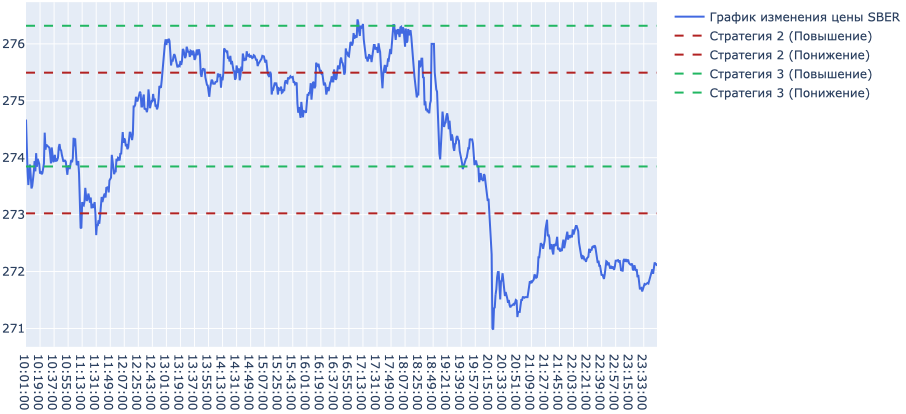
\includegraphics[keepaspectratio=true,scale=0.35]{images/chapter3/downdown.png}
        
        \caption{$s_2$ продажа в конце дня, $s_3$ продажа на понижение}
        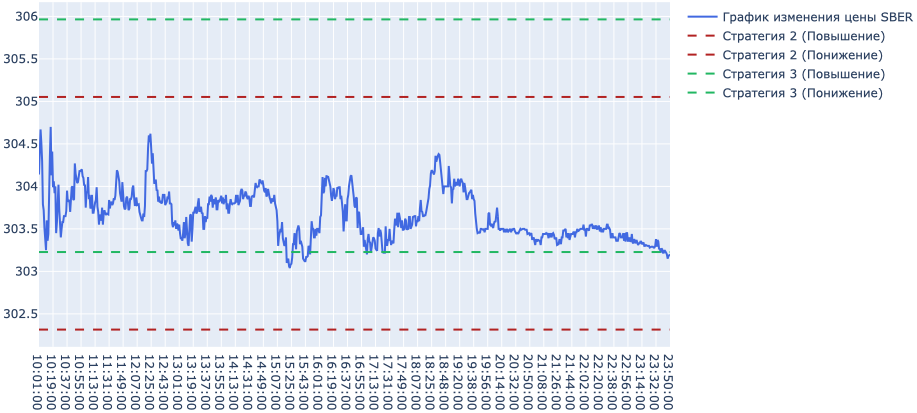
\includegraphics[keepaspectratio=true,scale=0.35]{images/chapter3/zerodown.png}
        
        \caption{$s_2$ продажа в конце дня, $s_3$ продажа в конце дня}
        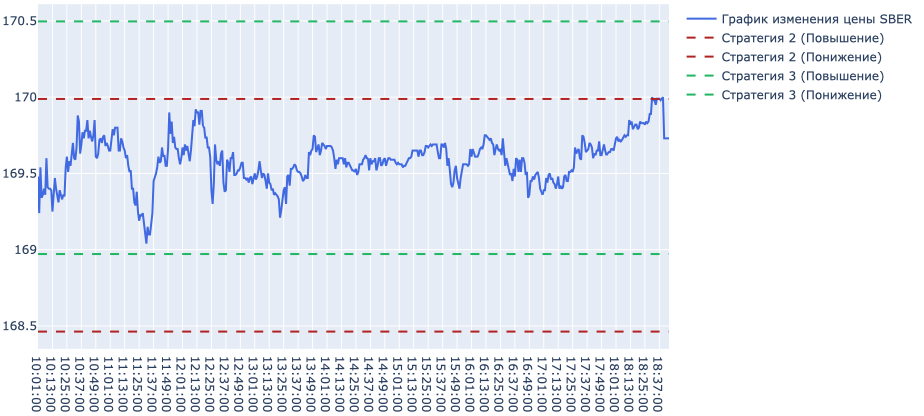
\includegraphics[keepaspectratio=true,scale=0.35]{images/chapter3/zerozero.png}
    \end{figure}
\end{center}


На этом численный эксперимент можно считать законченным. Подведем выводы по проделанной работе в следующей главе.



\chapter{Разбор парсинга данных на языке Python}

Приведем код на языке Python для предобработки и анализа данных. Для более удобного анализа и представления результатов я использовал Jupyter Notebook (в целом это может быть и другая интегрированная среда разработки для языка программирования Python). 
\smallskip
\smallskip

Считывание файлов и подключение библиотек: 
\lstinputlisting[language=Python]{listings/chapter4/code1.py} 

Функция для получения прибыли от стратегий и сравнения двух стратегий:

\lstinputlisting[language=Python]{listings/chapter4/code2.py} 

Функции для составления сводной таблицы для трех стратегий за все года. Вывод - это таблицы, которые были приведены в предыдущей главе:

\lstinputlisting[language=Python]{listings/chapter4/code3.py} 

Делаем вывод таблицы (приведем пример для стандартных значений функции):

\lstinputlisting[language=Python]{listings/chapter4/code4.py} 

Код для отрисовки поведения стоимости акций в пределах суток (они также были приведены в предыдущей главе)

\lstinputlisting[language=Python]{listings/chapter4/code5.py} 
\chapter{Список используемых ресурсов}

\begin{enumerate}
\item[{[1]}] Токарев С.С., "Нетранзитивный лохотрон" на фондовом рынке. Об одной перспективной форме платного обучения экономике, 2009.
\item[{[2]}] Grimmett, Geoffrey R.; Stirzaker, David R., Probability and Random Processes (3rd ed.). Oxford University Press. p. 491, 2001
\item[{[3]}] \href{https://www.finam.ru/profile/moex-akcii/sberbank/export/}{Финам, Мосбиржа, акции Сбербанк, 2021.}

\end{enumerate}



\end{document}
% -----------------------------------------------------------------
